\documentclass[a4paper]{article}

\usepackage{amsmath}
\usepackage{parskip}
\usepackage{listings}
\usepackage{siunitx}
\usepackage{cleveref}
\usepackage{graphicx}
\usepackage{grffile}

\title{The Synapse Driver Defect Detection Tool (SD3T)}
\author{Sebastian Schmitt}
\date{December 2014}

% \newcommand{\func}[1]{\texttt{#1}}
\newcommand{\func}[1]{\lstinline!#1!}
\newcommand{\pkg}[1]{\lstinline+#1+}

\begin{document}

\maketitle

\tableofcontents

\section{Introduction}

This document describes the Synapse Driver Defect Detection Tool (SD3T)
originally developed by Sebastian Billaudelle~\cite{bachelor:SB}.

\section{Organization of the Software}

\begin{description}
  \item[defects.py] Aquires spikes (the only online part)
  \item[ana\_defects.py] Categorizes spikes and synapse drivers
  \item[plot\_defects.py] Makes plots
  \item[blacklist.py] Finds good neurons
  \item[shallow.py] Configures hardware
\end{description}

\section{Hardware Configuration}

\subsection{Global}

The following properties are configured for the full run:

\begin{itemize}
\item Wafer
\item HICANN
\item Background ISI\footnote{inter-spike interval}
\item HICANN frequency
\end{itemize}

Also the path to the calibration data can be given if other than the
default configuration should be used. The synapse drivers under test
can also be given.

\subsection{Routing}

The 224 synapse drivers on a HICANN are enumerated from 0 to
223. Drivers on the top half have numbers $d \in (0, 111)$, drivers on
Ithe bottom half are numbered $d \in (112,223)$.

On the top half, odd (even) drivers are on the left side (right) side,
while on the bottom half, odd (even) drivers are located on the right
(left) side.

From driver to bus, \func{shallow.get_bus_from_driver}:
%
\begin{equation}
  \text{bus} = \begin{cases}
    (\text{driver}/2)\bmod 8 & \text{top},\\
    7 - (\text{driver}/2)\bmod 8 & \text{bottom}.
  \end{cases}
\end{equation}

Dividing the integer driver number maps odd numbers to the nearest
smaller even number ($1\rightarrow 0$, $3\rightarrow 2$, \ldots).

The sending repeater number, i.e.\ the horizontal line, as function of the bus:
\begin{equation}
  % 0 -> 62
  % 1 -> 54
  % 2 -> 42
  % 3 -> 38
  % ...
  h_{\text{line}} = 8 \cdot (8 - \text{bus}) - 2
\end{equation}

The first vertical line for a given bus:
\begin{equation}
  v_{\text{line}} =
  \begin{cases}
    4\cdot\text{bus} & \text{left},\\
    159 - 4\cdot\text{bus} & \text{right}.
  \end{cases}
\end{equation}

\subsection{Neurons}

For unconnected denmems, top drivers can only stimulated neurons with
neuron number $n \in (0, 255)$. Bottom drivers neurons $n \in (256,
511)$. Neurons that are located on the output buffer that is used for
L2 input are excluded, i.e.:
\begin{equation}
  n \notin
  \begin{cases}
    (0+32\cdot\text{bus}, 32+32\cdot\text{bus})  & \text{top},\\
    (0+32\cdot\text{bus}+256, 32+32\cdot\text{bus}+256) & \text{bottom}
  \end{cases}
\end{equation}
\func{defects.get_neurons}.

Neuron fire with address $\in (0, 63)$.

\subsection{Synapse Driver and Synapse Array}

\begin{figure}
  \centering
  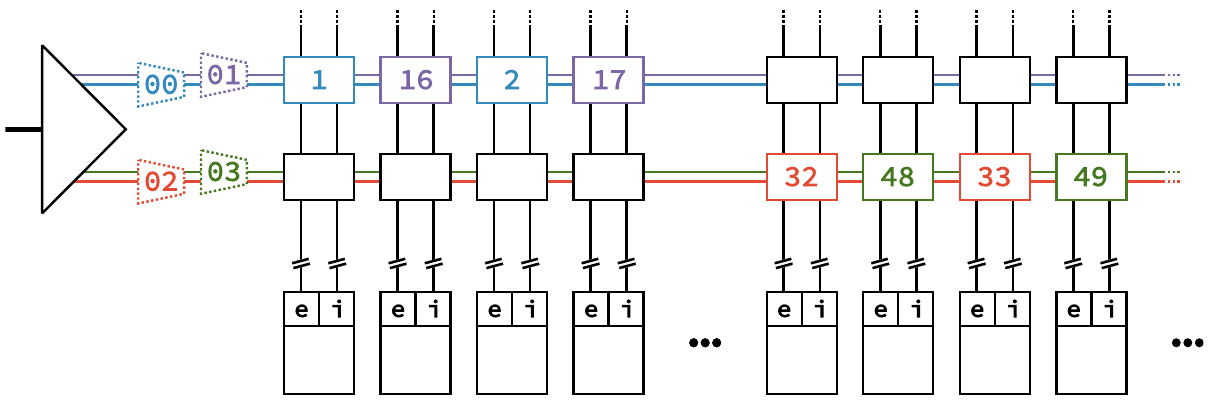
\includegraphics[width=\textwidth]{figures/syndrv_cfg}
  \caption{Synapse driver and synapse array configuration scheme.}
  \label{fig:syndrv_cfg}
\end{figure}

Every synapse driver steers two rows of synapses, top and
bottom\footnote{not related to top and bottom of the HICANN}. Each row
in turn has synapses that are connected to even and odd denmems. These
synapses are collectivly called a half-row. The synapses decode only
the four lower bits of the 6~bit address. The remaining two most
significant bits (MSBs) are decoded by the driver and define the
address range a half-row can handle.

The four different MSBs values, $0,1,2,3$, have to be exclusively
assigned to a top or bottom synapse row and even or odd neurons,
\func{defects.get_half_and_bank}, see \cref{fig:syndrv_cfg}.

All drivers, i.e.\ the decoders and the synapse array, can be
configured before the experiment is started,
\func{defects.prepare_drivers}.

For simplicity, a neuron emits the address that it is also configured
to be stimulated by.

\subsection{Merger Tree}

One output buffer to one GBit link, no merging except for background.

\subsection{Stimulation Pattern}

For each address a burst of spikes is injected with the following
properties:

\begin{tabular}{rl}
  Start offset & \SI{5}{\micro\second}\\
  Address offset & \SI{50}{\micro\second}\\
  Inter-spike interval & \SI{0.1}{\micro\second}\\
  Number of input spikes & 200
\end{tabular}

The start offset is a global offset. The address offset is added
multiplied with the stimulated address. The input spikes are send
with the configured interval.

\subsection{Running}
\label{sec:running}

Most of the configuration has to be programmed only once, e.g.\
floating gates and synapse array is unchanged during the sweep over
synapse drivers. Only the L1 routing has to be changed according to
the driver under test.

There is also no need to pull a reset. However, it is observed that
the time stamps of the spikes are off in the case off in the case of
no reset. This has to be taken into account for the categorization of
correct and incorrect spikes.

\section{Persistency}

The neo library~\cite{neo} is used with the HDF5 backend.

One block corresponds to one run over, usually all, synapse
drivers. Within the block, there is one segment for every driver. The
segment holds the spike trains for the recorded neurons.

Neo's annotation mechanism is used to store meta information, e.g.\
the annotations of the block contain the time of the experiment, the
wafer and HICANN used, as well as the frequency and the background
generator ISI\@. In the annotations of the segments, the current L1
voltages are stored. The result of the analysis is also partially
stored in the annotations.

Using Neo it is possible to read the contents lazy, i.e.\ only when
the data is really needed. This makes it possible to iterate
efficiently only over the annotations if the full information is not
necessary.

\section{Analysis}

\begin{figure}
  \centering
  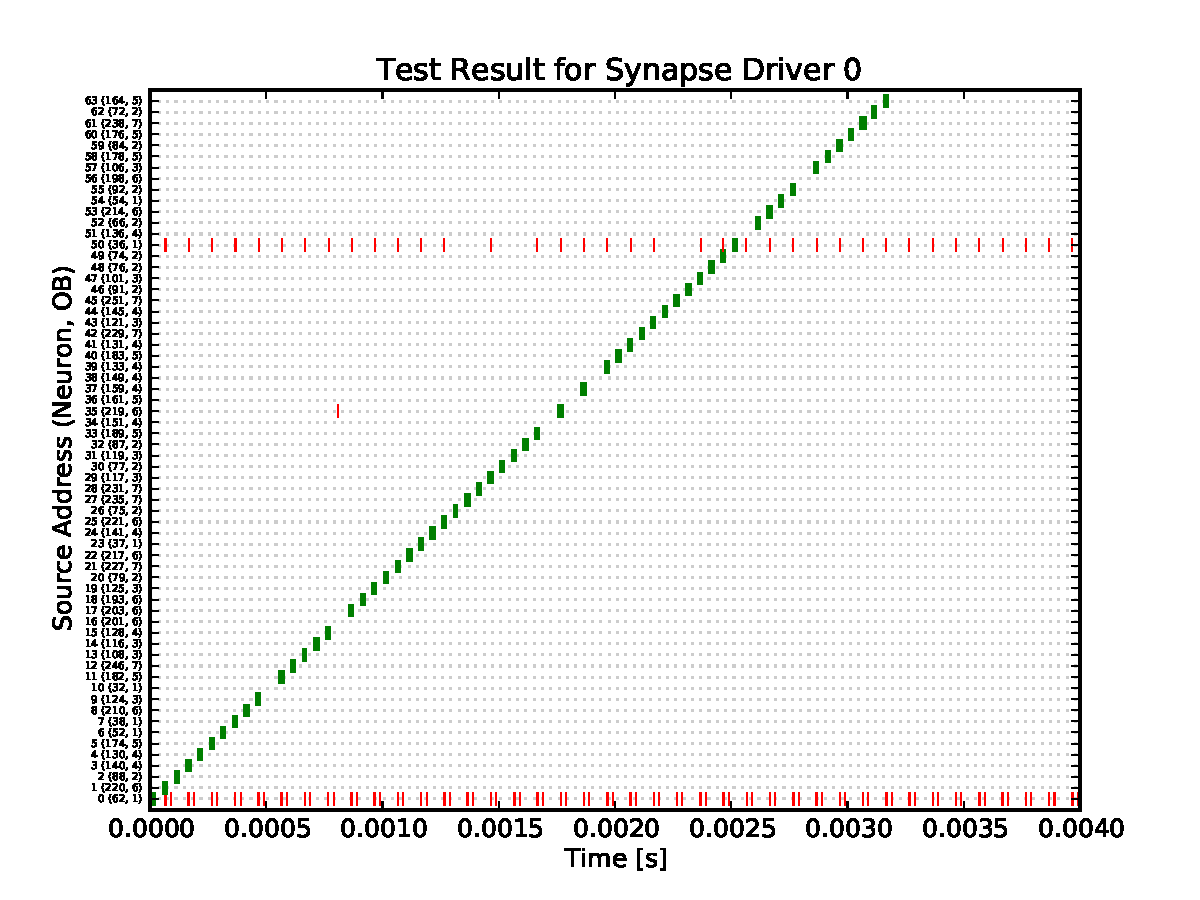
\includegraphics[width=0.5\textwidth]{figures/defects_bus_0_hline_62_vline_191_drv_0_w1_h288_f100_bkgisi10000_20140911_0.88_1.05}%
  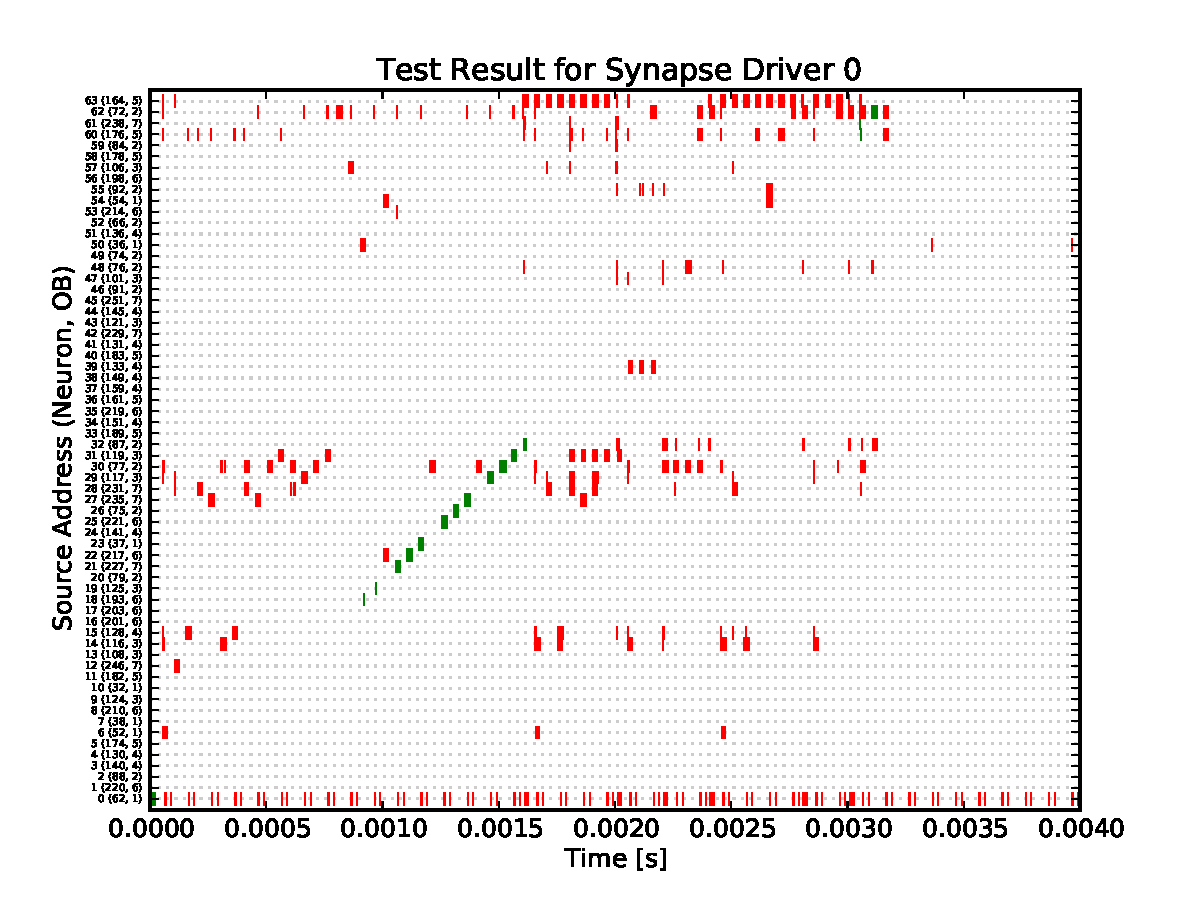
\includegraphics[width=0.5\textwidth]{figures/defects_bus_0_hline_62_vline_191_drv_0_w1_h288_f100_bkgisi10000_20140911_0.50_0.70}
  \caption{Example for analysis result.}
  \label{fig:ana_example}
\end{figure}

The analysis is split into two stages. In the first stage, the spikes
are categorized in correct and incorrect spikes. This is done by
\pkg{ana_defects.py} either standalone or on-the-fly while running
\pkg{defects.py}.


From the structure of the spike train it is known when spikes from a
neuron are expected. However, because of the problem with the time
stamps in the case of no reset discussed in \cref{sec:running}, the
window for correct spikes is enlarged by a safety factor of 3. The
number of correct and incorrect categorized spikes per address is
stored in the annotations of the segments.

\pkg{ana_defects.py} is also used to create plots
for visual inspection, see \cref{fig:ana_example}.

In the final stage of analysis, performed by \pkg{read_defects.py},
each driver is classified as either ``good'' or ``bad''. The ratio of
the total number of correct and incorrect spikes is used as
criterion. The spikes for address 0 are excluded because they will
always contain a high number of incorrect spikes originating from the
background events.

The driver is ``good'' if the correct to incorrect ratio exceeds
$0.8$. If there are no incorrect spikes but correct spikes, the driver
is also ``good''. If there are no spikes at all, the driver is
``bad''.  This simple criterion prooved to be sufficient if neurons
that always spikes are excluded.

The number of good drivers as well as the averaged L1 voltages are
stored in a json file.

\begin{thebibliography}{99}
  \bibitem{neo} Neo library
  \bibitem{bachelor:SB} Sebastian Billaudelle: Characterisation and
    Calibration of Short Term Plasticity on a Neuromorphic Hardware
    Chip
\end{thebibliography}

\end{document}

